% !TeX spellcheck = it_IT
% !TEX TS-program = pdflatex
% !TEX root = ../main.tex


% ********************************************************************
\section{Prototipo}
\label{sec:prototipo}
% ********************************************************************

La piattaforma proposta

\subsection{Login e autenticazione}





\subsection{Dashboard donatore}


%\begin{figure}[h]
%	\centering
%	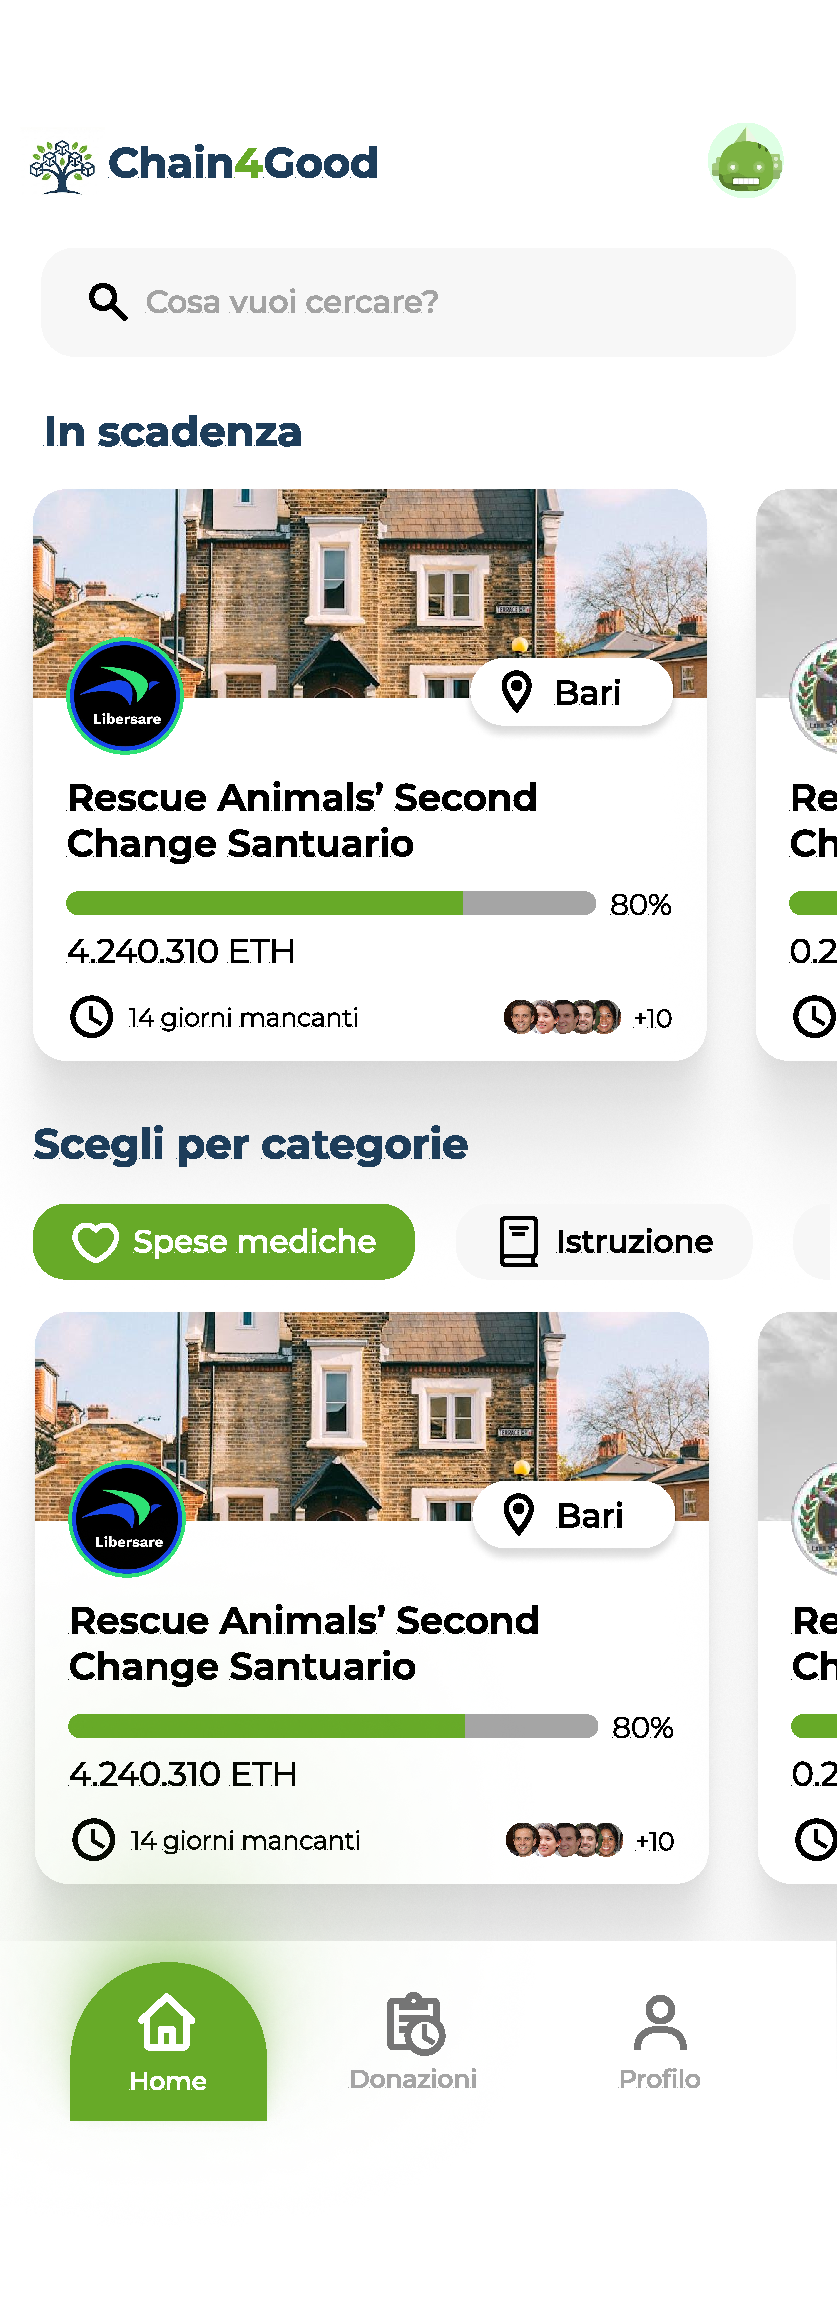
\includegraphics[width=0.45\textwidth]{images/home_utente.pdf}
%	\caption{Dashboard del donatore}
%	\label{fig:dashboard-donatore}
% \end{figure}


\subsection{Creazione progetto}
La creazione di un nuovo progetto (\ref{fig:Inserimento progetto}) richiede l'inserimento di




%\begin{figure}[h]
%	\centering
%	\begin{minipage}{0.46\textwidth}
%		\centering
%		\includegraphics[width=\textwidth]{images/nuovo_progetto1.pdf}
%	\end{minipage}
%	\hspace{0.9cm}
%	\begin{minipage}{0.46\textwidth}
%		\centering
%		\includegraphics[width=\textwidth]{images/nuovo_progetto2.pdf}
%	\end{minipage}
%	\caption{Inserimento di un nuovo progetto}
%	\label{fig:Inserimento progetto}
%\end{figure}





\subsection{Inserimento e valutazione spesa}
A differenza dei sistemi centralizzati in cui l'Ente ha piena e immediata disponibilità del \textit{budget}, l’architettura proposta prevede che i fondi raccolti rimangano vincolati all'interno di uno \textit{Smart Contract}. Per accedere a tali risorse, il beneficiario deve formalizzare una "Richiesta di Spesa" basata sull’inserimento dei seguenti parametri (\ref{fig:valutazione-spesa}): identificativo della spesa, importo richiesto, finalità e preventivo. \\
Una volta sottomessa, i donatori possono analizzare la documentazione ed esprimere un parere favorevole o contrario.

\subsubsection{Meccanismo di validazione}
Per garantire l'operatività del sistema ed evitare lo stallo decisionale, lo \textit{Smart Contract} è programmato per agire secondo le seguenti regole:
\begin{itemize}
	\item La richiesta è approvata se la maggioranza dei votanti esprime un parere favorevole.
	\item Qualora non venga registrata alcuna attività di voto entro il termine stabilito, la richiesta viene approvata automaticamente.
	\item In presenza di una partecipazione parziale, la soglia di maggioranza viene ricalcolata in funzione dei voti espressi, garantendo che la decisione finale rispecchi la volontà della parte attiva della comunità.
\end{itemize}

Solo al raggiungimento dei criteri di approvazione, lo \textit{Smart Contract} esegue automaticamente il trasferimento della somma richiesta al \textit{Wallet} del beneficiario.



\begin{figure}[h]
	\centering
	\begin{minipage}{0.46\textwidth}
		\centering
		\includegraphics[width=\textwidth]{images/nuova_spesa.pdf}
	\end{minipage}
	\hspace{0.9cm}
	\begin{minipage}{0.46\textwidth}
		\centering
		\includegraphics[width=\textwidth]{images/valutazione_spesa.pdf}
	\end{minipage}
	\caption{Valutazione di una richiesta di spesa}
	\label{fig:valutazione-spesa}
\end{figure}

